\documentclass{article}
\usepackage{bookmark}
\usepackage{color}
\usepackage{amsmath}
\usepackage{hyperref}
\usepackage{listings}
\usepackage{xcolor}
\usepackage{indentfirst}
\usepackage{graphicx}
\usepackage{amsfonts}
\usepackage{hyperref}
\usepackage[top=2cm, bottom=2cm, left=2cm, right=2cm]{geometry}  
\usepackage{algorithm}  
\usepackage{algorithmicx}  
\usepackage{algpseudocode}
\pagestyle{headings}
\markright{\large Zhang Yichi 516370910260\hfill VE477 h8\hfill}
\renewcommand{\algorithmicrequire}{\textbf{Input:}}  
\renewcommand{\algorithmicensure}{\textbf{Output:}}  

\begin{document}
{\noindent {\bf Ex 1.} PART I. 1. The graph is shown below\\

\begin{figure}[h]
    \centering
    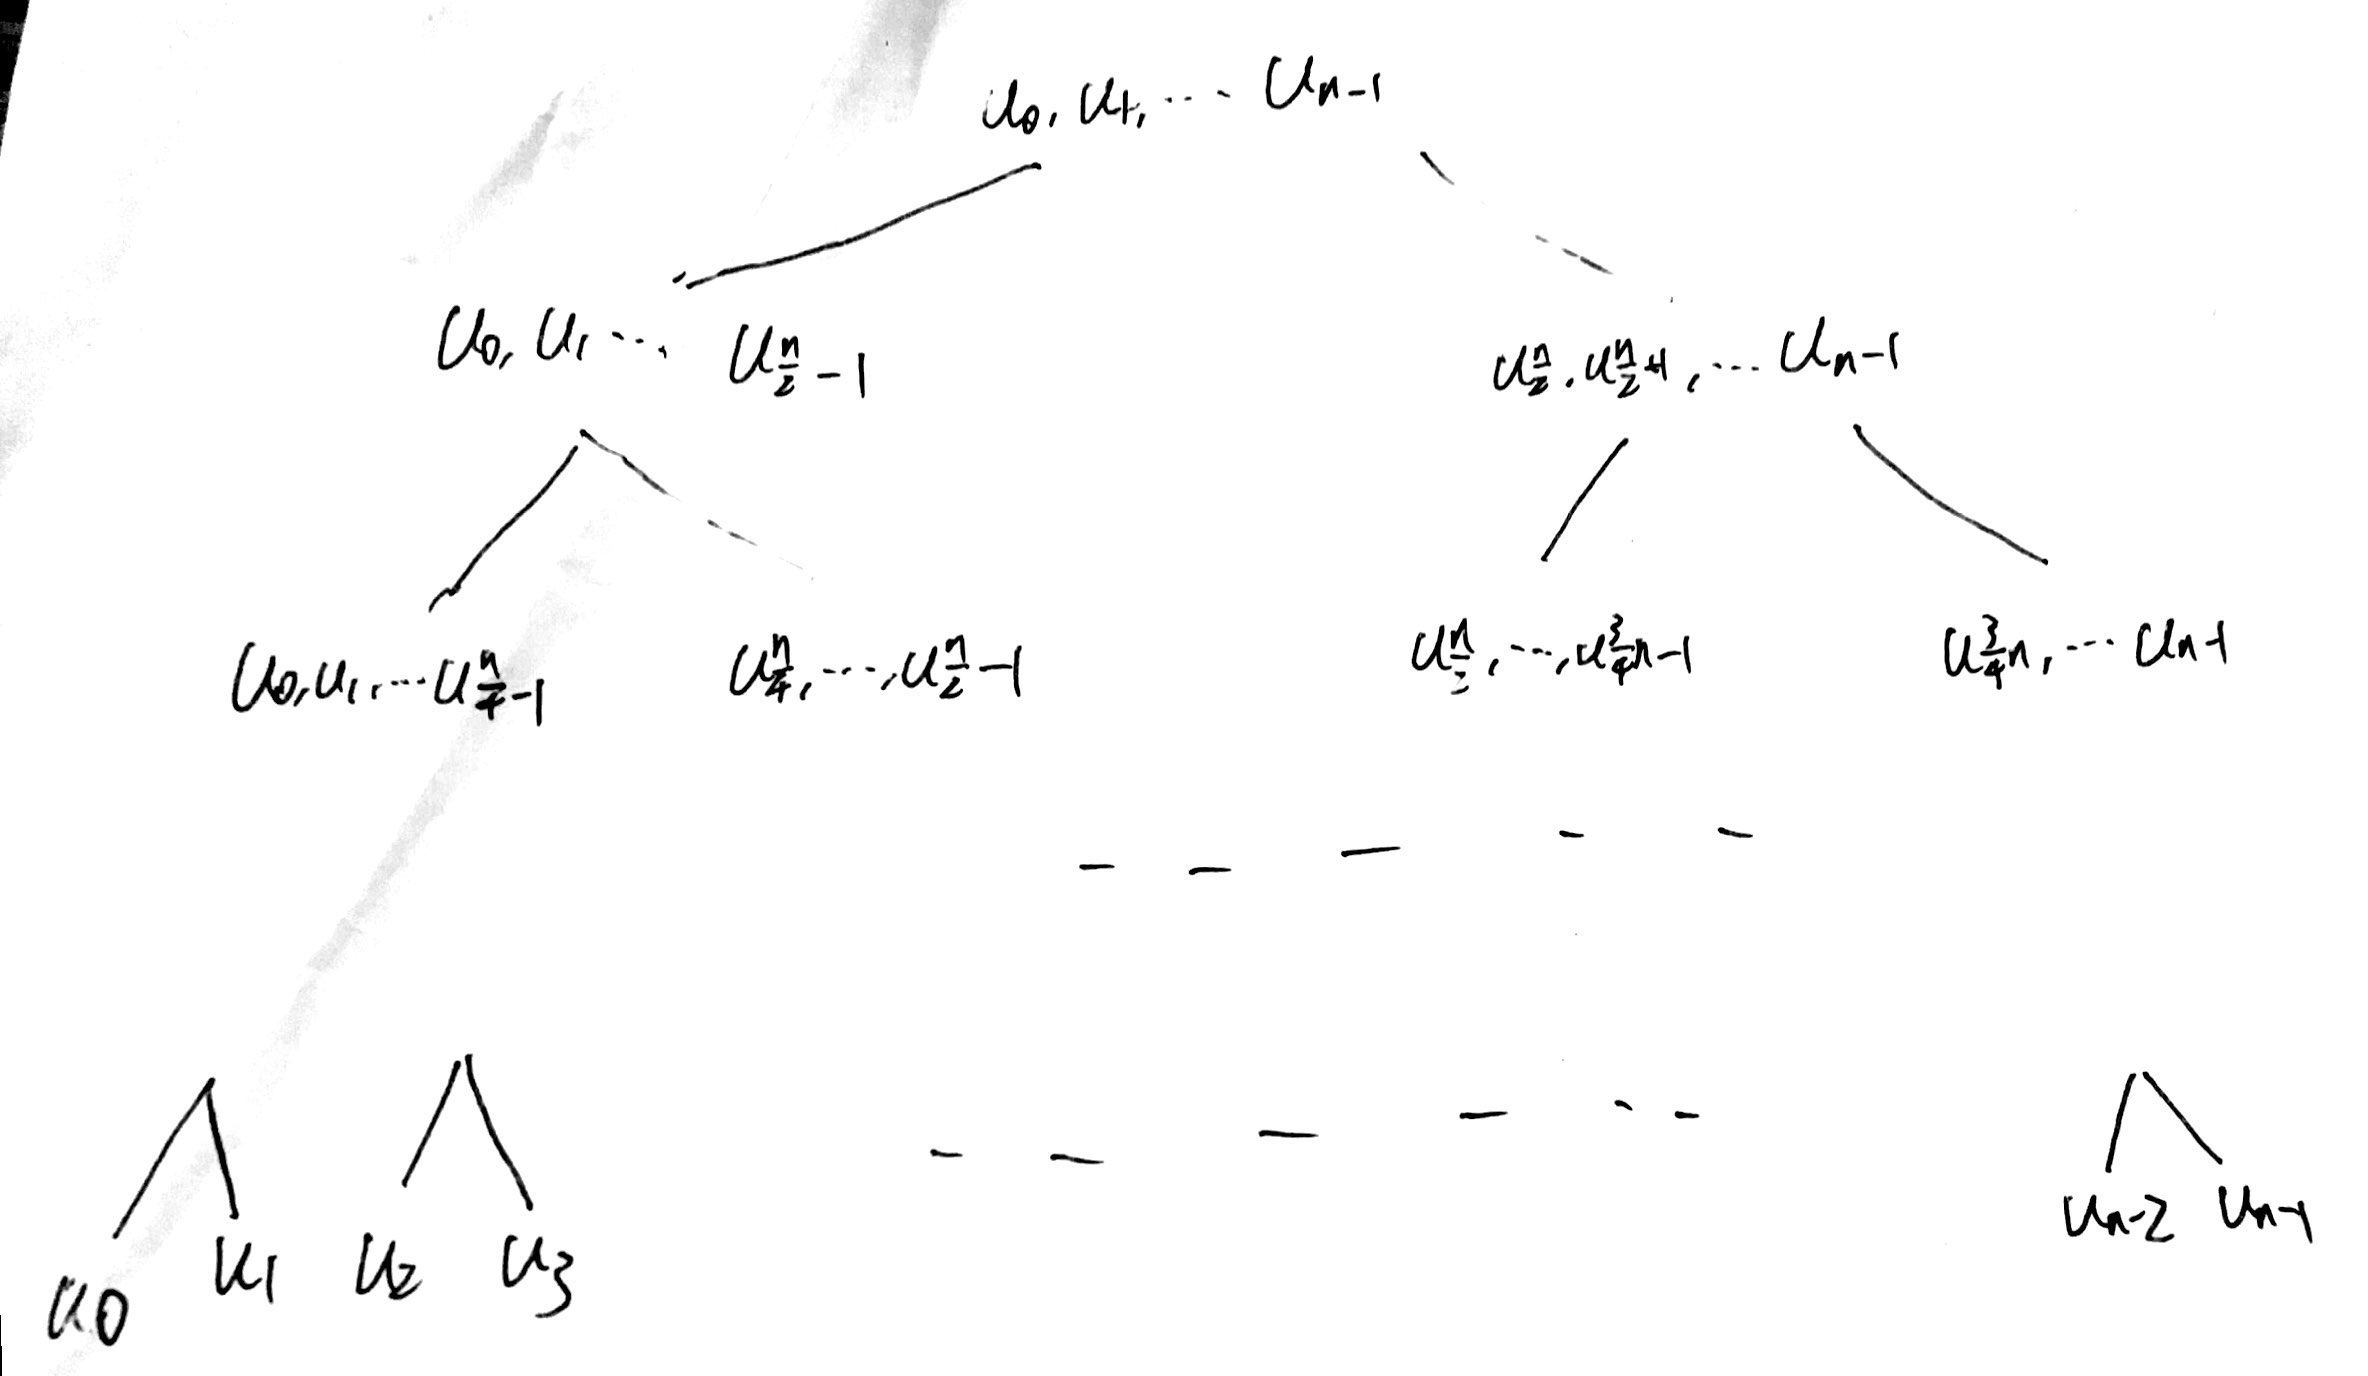
\includegraphics[scale=0.1]{1.jpg}
\end{figure}

{\noindent 2. Fisrst, see $M_{0,j} = \prod_{l=0}^0m_{j+l} = m_j$}

Next, see $M_{i+1,j} = \prod_{l=0}^{2^{i+1}-1}m_{j{2^{i+1}}+l} = \prod_{l=0}^{2^i-1}m_{2j2^i+l}\times \prod_{l=2^i}^{2^{i+1}-1}m_{2j2^i+l} = M_{i,2j}(\prod_{l=0}^{2^i-1}m_{(2j+1)2^i+l}) = M_{i,2j}M_{i,2j+1}$


{\noindent 3. $M_{i,j}$ should lie on the $i_{th}$ layer from the bottom, and $j_{th}$ node from the left\\}

{\noindent 4. (a) The algorithm is shown below.}

\begin{algorithm}[H]
    \caption{Make Subproduct}  
    \begin{algorithmic}[1] 

        \Require $n-2^k$,$\{u_0,u_1,...u_{n-1}\}$
        \Ensure Subproducts $M_{i,j}$

        \For {$i\gets 0 \to n-1$}
            \State $M_{0,i}\gets X-u_i$
        \EndFor

        \For {$i\gets 1 \to k$}
        \For {$j\gets 0 \to 2^{k-i}-1$}
            \State $M_{i,j}\gets M_{i-1,2j}M_{i-1,2j+1}$
            \EndFor
        \EndFor
    \end{algorithmic}  
\end{algorithm}

{\noindent (b) The algorithm is shown below.}
\begin{algorithm}[H]
    \caption{Fast Multipoint Evaluation}  
    \begin{algorithmic}[1] 

        \Require P,$n-2^k$,$\{u_0,u_1,...u_{n-1}\}$, subproducts $M_{i,j}$
        \Ensure Evaluation of $\{P(u_0),P(u_1),...,P(u_{n-1})\}$

        \Function{Dividedown}{$f,k,i$}
            \If {$n=1$}
                \State \Return f
            \EndIf
            \State $fleft \gets f \text{ mod } M_{k-1,2i}$
            \State $fright \gets f \text{ mod } M_{k-1,2i+1}$
            \State $leftset \gets DIVIDEDOWN(fleft,k-1,2i)$
            \State $rightset \gets DIVIDEDOWN(fleft,k-1,2i+1)$
            \State \Return $\{leftset,rightset\}$
        \EndFunction
        \State \Return $DIVIDEDOWN(P,k,0)$
    \end{algorithmic}  
\end{algorithm}

{\noindent 5. (a) If the tree has only one layer, which means that $f$ will just be a constant, and returning $f$ directly is surely true.}

Suppose that the values is correct for $k-1$ layers, consider the situation on $k_{th}$ layer.

Because we are doing modulus operation, so the true function $P$ can be written as $$P = qleft(u_i)M_{k-1,0}+rleft(u_i)$$ or $$P = qright(u_i)M_{k-1,1}+rright(u_i)$$

It can be seen that the $qM$ term will be $0$ for the value we want to use and so the true value will be in the $r$ term, which we evaluate using a $k-1$ layer tree, thus the correctness is proven.\\

{\noindent (b). The recurrance relation can be written as $T(n)=2T(n/2)+M(n)$, thus the complexity is $\mathcal{O}(M(n)\log{n})$\\}

{\noindent PART II 2. $m' = \sum_{i=0}^{n-1}(X-u_i)'\frac{m}{X-u_i} = \sum_{i=0}^{n-1}\frac{m}{X-u_i}$, and because all terms with $(X-u_i)$ will be zero in $m'$, the only term remains is $\frac{m}{X-u_i} = 1/s_i$}

{\noindent 3. The algorithm is given below}

\begin{algorithm}[H]
    \caption{Fast Interpolation}  
    \begin{algorithmic}[1] 

        \Require $n-2^k$,$\{u_0,u_1,...u_{n-1}\}$, $y = \{P(u_0),P(u_1),...,P(u_{n-1})\}$, subproducts $M_{i,j}$
        \Ensure $P$

        \Function{multiUp}{$f,k,i$}
            \If {$n=1$}
                \State \Return y
            \EndIf
            \State $fleft \gets MULTIUP(fleft,k-1,2i)$
            \State $fright \gets MULTIUP(fleft,k-1,2i+1)$
            \State \Return $fleft\times M_{k,1}+fright\times M_{k,0}$
        \EndFunction
        \State \Return $MULTIUP(P,k,0)$
    \end{algorithmic}  
\end{algorithm}

{\noindent 5. The recurrance relation can be written as $T(n)=2T(n/2)+M(n)$, thus the complexity is $\mathcal{O}(M(n)\log{n})$\\}

{\noindent 6. The calculation is correct, but there might need much space to do this job.\\}

\hrule

\vskip 2em

{\noindent {\bf Ex 2.} 2. Let us check this dialogue sentence by sentence, an we pay more attention on the logic of $S_1$\\

\begin{itemize}
    \item S1 : ``I’m not surprised, I knew you couldn’t know!"
    
    It means that in $S_1$'s mind, however you decompose his sum, you can never have a product that can be uniquely factored in this scenario.

    This sentence can exclude most of the possibilities of the sum. First, every number larger than 54 can be excluded, because those sums can all be possibly decomposed as $53+x$, and if $S_2$ has $53x$, he can guess it because you can only have 53 as an individual factor.

    Next, all sums that can be decomposed to two primes can be excluded. There are mainly two cases: $2+prime$ or $oddprime+oddprime$. For $2+prime$, we can exclude $4,5,7,9,13,15,19,21,25,31,33,39,43,45,49$. And for $oddprime+oddprime$, actually we can exclude all even numbers, based on the famous Goldbach's conjecture ( we can assume that it is correct in such a small range ). In that case, what we have now are $11,17,23,27,29,35,37,41,47,51,53$

    Consider the case of $51$, it is possible that the two numbers are $17$ and $34$. In that case the product will be $2\times 17^2$, and the only possibility is $17$ and $34$, so it can also be excluded.

    \item S2 : ``Uhm ... so now I know ..."
    
    When he heard that what $S_1$ said, he will compress the range of sums into what we concluded. And as he knew it, it means that although his product has multiple kinds of decompositions, only one of the possible sum falls in this set.

    \item S1 : ``So do I!"
    
    It means that the answer of $S_2$ will not confuse $S_1$. In this way we can exclude those whoe can be decomposed to $2^n+p$(p is prime) in more than one ways. Because when $S_2$ has $2^np$ and he gets what $S_1$ said, he know that the only possibility is $2^n+p$, but $S_1$ still is not able to decide from $2^{n_1}+p_1$ and $2^{n_2}+p_2$. Then the remaining are $17,29,41,53$, and now we see it one by one.

    Consider the case $29 = 2+27 = 4+25$, and in both cases $S_2$ can then know while $S_1$ still cannot judge.

    $41 = 4+37 = 10+31$, same

    $53 = 6+47 = 16+37$, same.

    So the only case is $17 = 13+4$, the two numbers are $13$ and $4$

    {\noindent 3. In fact the word "if they collide they all go reversely" is of no use.Because all ants are the same, the situation should be the same as the situation when the cable is wide enough that both ants can pass each other when they meet. So the maximum total time should still be 1s}
\end{itemize}


\end{document}